\chapter{Sintesi dell'MTBE}
L'MTBE\footnote{Metil \textit{Terz}-Butil Etere} � una sostanza che negli ultimi decenni ha subito un notevole sviluppo grazie ad alcune sue caratteristiche che lo hanno portato a sostituire il piombo tetraetile, sostanza altamente tossica poich� contiene un metallo pesante e nociva per i catalizzatori delle marmitte, come antidetonante nelle benzine. Il suo impiego in questo settore ha fatto si che la sua produzione sia stata quella a pi� alto tasso di crescita negli anni ottanta, portandolo a produzioni paragonabili a quelle delle olefine (etilene, propilene, ...), tanto da raggiungere la posizione 12 nelle \textit{top 50} delle sostanze pi� prodotti in USA nel 1995.

I vantaggi che hanno portato la scelta dell'MTBE come sostituto del \ce{Pb(Et)_4} nelle benzine sono duplici, da un lato l'utilizzo dell'MTBE porta ad un innalzamento del numero di ottano della miscela, permettendo di avere motori con rapporti di compressione maggiori e di conseguenza consumi ridotti fungendo anche da fornitore di ossigeno e migliorando la combustione. Altro fattore rilevante per la scelta di questa sostanza � il costo di produzione che non � totalmente legato al valore del greggio (il prezzo dipende anche dal metanolo, prodotto a basso costo). Come fornitore di ossigeno nella miscela possono essere utilizzate anche altre sostanze, quali alcoli (Etanolo, TBA\footnote{\textit{terz}-butanolo}), eteri (TAME\footnote{teramil-metil-etere}, TAEE\footnote{teramil-etil-etere}, DIPE\footnote{di-isopropil-etere}) con la differenza che questi hanno un costo maggiore e non aumentano il numero di ottano quanto l'MTBE. Da considerare che le benzine riformulate (in America pari a circa il 32\% della benzina erogata) � obbligatoria una presenza di ossigeno pari al 2\%, ma per raggiungere tali valori � necessario che sia presente l'11\% di MTBE; ci� pu� far capire l'importanza di questo prodotto, che in America � passato da 10MTPY\footnote{Milion Tons Per Year = milioni di tonnellate annue} del 1991 al 24MTPY del 1996 con un treand in continua crescita. Negli anni '90 si � scoperto in California (USA), dove l'uso di MTBE � massiccio e pari a circa il 40\% del consumo americano, che questa sostanza pu� provocare inquinamento delle falde acquifere, essendo scarsamente biodegradabile; per questo motivo, e una sua presnta tossicit�, negli ultimi anni si sta cercando un degno sostituto.

\section{Sintesi}
\subsection{Il meccanismo di reazione}
La sintesi dell'MTBE � abbastanza semplice, infatti si tratta di una reazione in cui del metanolo e dell'isobutene vengono miscelati in presenza di un catalizzatore acido. Questo lega a se l'\ce{iso-butene} scindendo il doppio legame e creando cos� una parziale carica positiva. L'ossigeno del metanolo possiede due doppietti elettronici liberi che hanno cariche parziali negative, di conseguenza viene attratto dall'isobutano legato al catalizzatore e si ha formazione dell'MTBE.

La reazione complessiva � moderatamente esotermica ($\Delta H$= -10Kcal/mol) e controllata dall'equilibrio; per questo motivo si opera a temperature sufficientemente basse (circa $50-80^oC$) e con una pressione di qualche atmosfera cos� da mantenere l'MTBE in fase liquida ($T_{eb} = 82^oC$).

I sottoprodotti che si possono formare sono eteri dimetilici dalla condensazione di due molecole di metanolo, il \ce{di-iso-butene} dalla reazione di due molecole di butene e l'alcool terz-butilico.

\subsection{L'impianto}
Come reagenti vengono utilizzati le miscele di \ce{C_4} e metanolo, poich� la selettivit� verso l'isobutene � talmente elevata da permettere di avere comunque una purezza spinta e una conversione dell'\ce{iso-butene} praticamente unitaria. Si ha, quindi, una prima zona in cui avviene il lavaggio della frazione \ce{C_4} (gi� privata del butadiene) con acqua per eliminare eventuali impurezze che possono danneggiare il catalizzatore, una seconda zona in cui avviene la reazione tra \ce{iso-butene} e \ce{metanolo} e la successiva separazione dell'MTBE dai gas rimanenti. La separazione prosegue estraendo il metanolo non reagito con acqua e facendo seguire il tutto da uno stripper (o rettifica) per ottenere la separazione del metanolo dall'acqua di estrazione.

La zona di reazione � composta da due reattori, il primo in cui avviene il grosso della produzione di MTBE a cui segue una colonna di separazione per estrarre il grosso dell'MTBE e un secondo di raffinazione del processo in cui si ha la completa conversione dell'\ce{iso-butene}. Lo schema � rappresentato in \figurename~\ref{fig:mtbe:Plant}.

\begin{figure}[htbp]
	\centering
		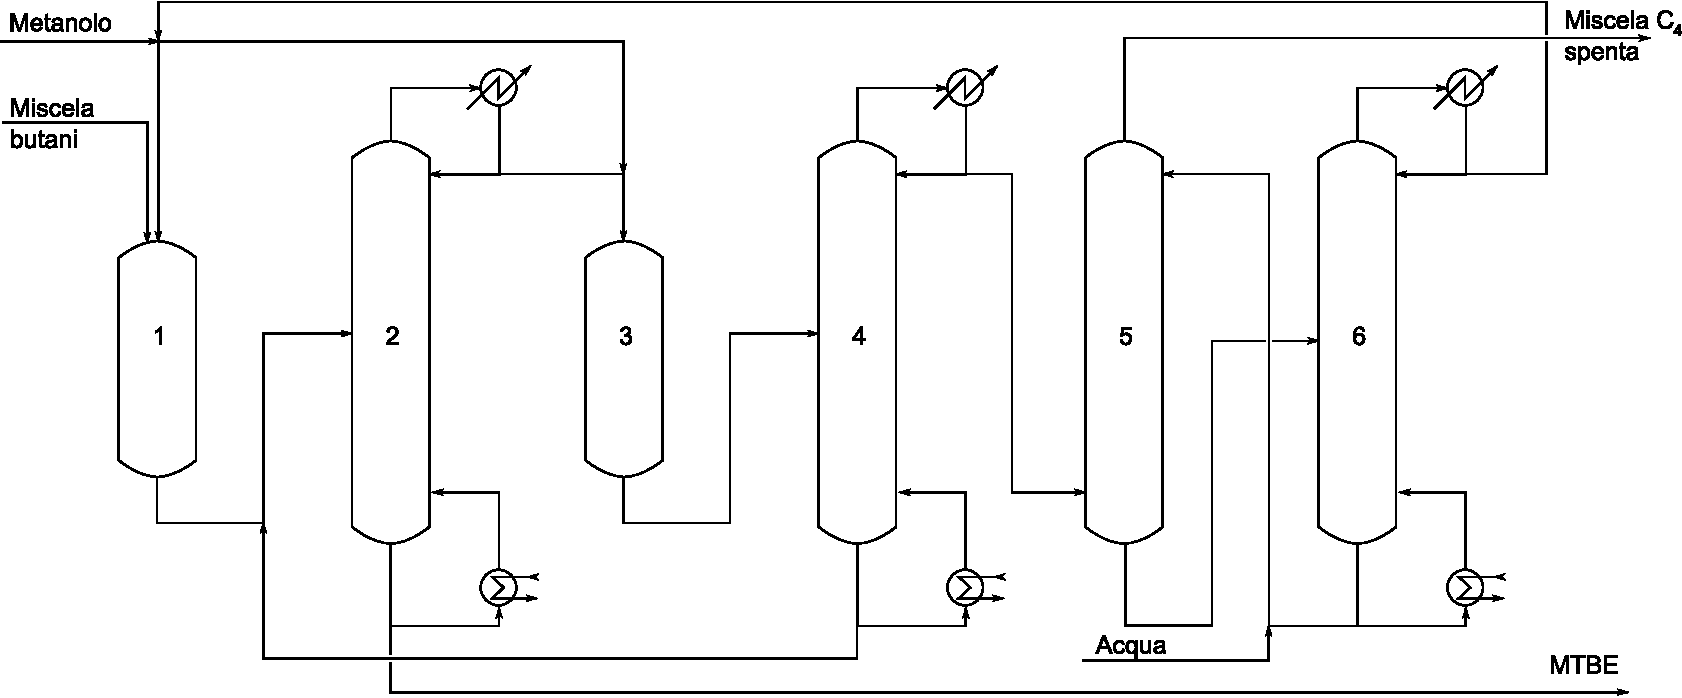
\includegraphics[width=0.95\textwidth]{image/mtbePlant}
	\caption[Schema dell'impianto per la produzione di MTBE]{Schema dell'impianto per la produzione di MTBE. 
	\textit{1}: Primo reattore;
	\textit{2}: Rettifica per la separazione dell'MTBE;
	\textit{3}: Secondo reattore;
	\textit{4}: rettifica per recupero MTBE;
	\textit{5}: Colonna di lavaggio con acqua;
	\textit{6}: Separazione metanolo-acqua;
	}
	\label{fig:mtbe:Plant}
\end{figure}

\subsection{I reattori}
La produzione di MTBE pu� avvenire in diverse tipologie di reattori, attualmente le tipologie utilizzate sono le quattro elencate di seguito.

\subsubsection{Reattore adiabatico}
E' il reattore pi� semplice da realizzare, inizialmente si ha una rapida crescita della temperatura parallela alla conversione dei reagenti in MTBE, fino a quando non viene raggiunto un punto di equilibrio. Il reattore deve essere sovra dimensionato per ovviare ai problemi di disattivazione del catalizzatore, inoltre la parte inattiva � sottoposta alla massima temperatura operativa. Da notare che in questo modo si ha la formazione notevole di sottoprodotti, quindi � da prevedere una zona dell'impianto per la purificazione del prodotto desiderato da questi.

\subsubsection{Reattore a scambio termico}
Si tratta di un reattore simile ad uno scambiatore di calore, dove all'interno dei tubi e si trova il catalizzatore e vengono fatti passare i reagenti, mentre dall'esterno (lato shell) si ha il passaggio del refrigerante utilizzato, che pu� essere condotto in equi o controcorrente. Da valutare in fase di ideazione se utilizzare un flusso equicorrente (si favorisce lo scambio termico dove le condizioni sono pi� critiche), o usare un flusso controcorrente che garantisce all'uscita una temperatura inferiore (e di conseguenza una conversione pi� elevata).

Si tratta di un sistema ben pi� flessibile del reattore adiabatico inquanto permette di variare le condizioni operative in funzione dell'alimentazione.

\subsubsection{Reattore bollente}
Si tratta di un reattore simile ad una camera di flash adiabatico, il calore di reazione porta il sistema all'ebollizione, il che rende meno critico il problema del profilo termico, essendo l'intera miscela alla temperatura di ebollizione. La temperatura di ebollizione pu� essere regolata agendo sulla pressione del sistema e quindi � possibile un controllo sulle condizioni del sistema; di contro, invece, si ha che vi � una grande zona non utilizzata, infatti nella fase vapore, ricca dei componenti volatili, la reazione non procede rendendo di fatto inutilizzata quella zona di reattore.

\subsubsection{Colonna reattiva}
Pu� essere paragonata ad una serie di flash posti in cascata, dove la frazione liquida in uscita dallo stadio precedente (ricca di MTBE) viene inviata allo stadio seguente, in cui i reagenti formano altro MTBE. Con questa tipologia di reattore le rese sono notevolmente migliorate a fronte di una diminuzione di una drastica diminuzione dei sottoprodotti indesiderati.